%68
\begin{frame}
  A HTML szemantikus elemei az oldal funkcionális részeinek jelölésére:
  \begin{description}[m]
    \item[\texttt{<main>}] \hfill \\ A dokumentum legfőbb tartalmát jelöli, ami nem ismétlődik más oldalakon, azaz nem tartalmazza pl. a menüsort, oldal logot, szerzői jogi információt. \kiemel{Csak egyszer fordulhat elő} a dokumentumban! Nem lehet az \texttt{<article>}, \texttt{<aside>}, \texttt{<footer>}, \texttt{<header>}, \texttt{<nav>} leszármazottja. Célja: akadálymentesítés, Safari olvasó funkciója is ezt emeli ki.
    \item[\texttt{<nav>}] \hfill \\ Az oldal legfontosabb navigációs hivatkozásainak gyűjteménye, pl. menü, tartalomjegyzék. A menüt gyakran CSS formázott \texttt{<ul>} elemekkel valósítják meg. Több \texttt{<nav>} is lehet egy oldalon, pl. külön az oldalon belüli, és azon kívülre mutató hivatkozásoknak.
  \end{description} 
\end{frame}

%69
\begin{frame}
  \begin{description}[m]
    \item[\texttt{<article>}] \hfill \\ Az oldal többi részétől függetlenül, önmagában is értelmes tartalmi rész, pl. fórum- vagy blogbejegyzés, hír. Jellemzően címsorral kezdődik. Egy oldalon belül többször is előfordulhat, akár egymásba is ágyazhatók (pl. blogbejegyzés és az arra adott reakciók). A megjelenés dátumát gyakran tartalmazza beágyazott \texttt{<time>} elemmel (a \texttt{datetime} attribútummal gépek is felismerik).
    \item[\texttt{<section>}] \hfill \\ Dokumentum egy része, fejezete, de akár fejléce, lábléce is lehet. Ajánlott címsorral ellátni. Nem lehet az \texttt{<address>} leszármazottja.
  \end{description} 
\end{frame}

%70
\begin{frame}
  \begin{description}[m]
    \item[\texttt{<aside>}] \hfill \\ A tartalomhoz lazán kapcsolódó kiegészítés, megjegyzés. Akadálymentesítési okokból használják a \texttt{role} attribútumot.
    \item[\texttt{<header>}] \hfill \\ Általában a dokumentum bevezetőjét, navigációs hivatkozásokat tárol. Gyakran tartalmaz címsor (\texttt{<h1>}-\texttt{<h6>}) elemeket, logot, szerzőt. Többször is előfordulhat a dokumentumban, pl. több \texttt{<article>} elejében.
    \item[\texttt{<footer>}] \hfill \\ Egy dokumentum vagy fejezet lábléce. Jellemzően a szerző nevét, szerzői jogi információt, kapcsolatfelvétel módját (ld. \texttt{<address>}), oldaltérképet, impresszumot, stb. tartalmaz. Többször is előfordulhat egy dokumentumban (pl. minden \texttt{<article>} végén).
  \end{description} 
\end{frame}

%71
\begin{frame}
  \begin{exampleblock}{\textattachfile{reszek.html}{reszek.html}}
    \footnotesize
    \lstinputlisting[style=HTML,linerange={7-19},numbers=left,firstnumber=7]{reszek.html}
  \end{exampleblock}
\end{frame}

%72
\begin{frame}
  \begin{exampleblock}{\textattachfile{reszek.html}{reszek.html}}
    \footnotesize
    \lstinputlisting[style=HTML,linerange={20-26},numbers=left,firstnumber=20]{reszek.html}
    \lstinputlisting[style=HTML,linerange={34-37},numbers=left,firstnumber=34]{reszek.html}
  \end{exampleblock}
\end{frame}

%73
\begin{frame}
  \begin{exampleblock}{\textattachfile{reszek.html}{reszek.html}}
    \footnotesize
    \lstinputlisting[style=HTML,linerange={47-56},numbers=left,firstnumber=47]{reszek.html}
  \end{exampleblock}
\end{frame}

%74
\begin{frame}
  \begin{exampleblock}{\textattachfile{reszek.html}{reszek.html}}
    \footnotesize
    \lstinputlisting[style=HTML,linerange={103-115},numbers=left,firstnumber=103]{reszek.html}
  \end{exampleblock}
\end{frame}

%75
\begin{frame}
  Tartalom megjelenítése / elrejtése
  \begin{columns}[T]
    \column{0.67\textwidth}
      \begin{description}[m]
        \item[\texttt{<details>}] \hfill \\ Interaktív oldalrész, amit a felhasználó elrejthet/megjeleníthet (alapértelmezetten rejtett; megjeleníthető az \texttt{open} attribútummal). Gyakorlatilag bármi beleágyazható.
        \item[\texttt{<summary>}] \hfill \\ A blokk kattintható fejléce, mindig látszik.
      \end{description}
    \column{0.3\textwidth}
      \begin{exampleblock}{\textattachfile{reszletek.html}{reszletek.html}}
        
\includegraphics[width=\textwidth]{reszletek.png}
      \end{exampleblock}
  \end{columns}
\end{frame}

%76
\begin{frame}
  \begin{exampleblock}{\textattachfile{reszletek.html}{reszletek.html}}
    \footnotesize
    \lstinputlisting[style=HTML,linerange={9-14},numbers=left,firstnumber=9]{reszletek.html}
    \lstinputlisting[style=HTML,linerange={20-21},numbers=left,firstnumber=20]{reszletek.html}
  \end{exampleblock}
\end{frame}

%77
\begin{frame}
  A \textattachfile{c64.txt}{c64.txt} fájl felhasználásával készítse el a \texttt{c64.html} fájlt!
  \begin{itemize}
    \item Az újság neve és a rovatok kerüljenek a dokumentum fejlécébe!
    \item Készítsen navigációs sávot az \emph{index}, \emph{c64.com} és \emph{Wikipédia} elemekből!
    \item Az oldal \emph{fő} része tartalmazza a teljes cikket!
    \item A cikknek is legyen fejléce, ami a \emph{cikk címéből}, \emph{szerzőjéből} és a \emph{megjelenés idejéből} áll!
    \item Az \emph{,,Egy maroknyi dollárért''} és a \emph{,,Specifikáció''} legyen a cikk két fejezetének címe!
    \item A \emph{,,Microprocesszor''} és \emph{,,Video hardver...''} kattintásra jelenjen meg/tűnjön el!
    \item Az \emph{,,Önök írták''} legyen az ,,oldalsáv'' fejléce!
  \end{itemize}
\end{frame}

%78
\begin{frame}
  \begin{exampleblock}{\textattachfile{c64.html}{c64.html}}
    \centering 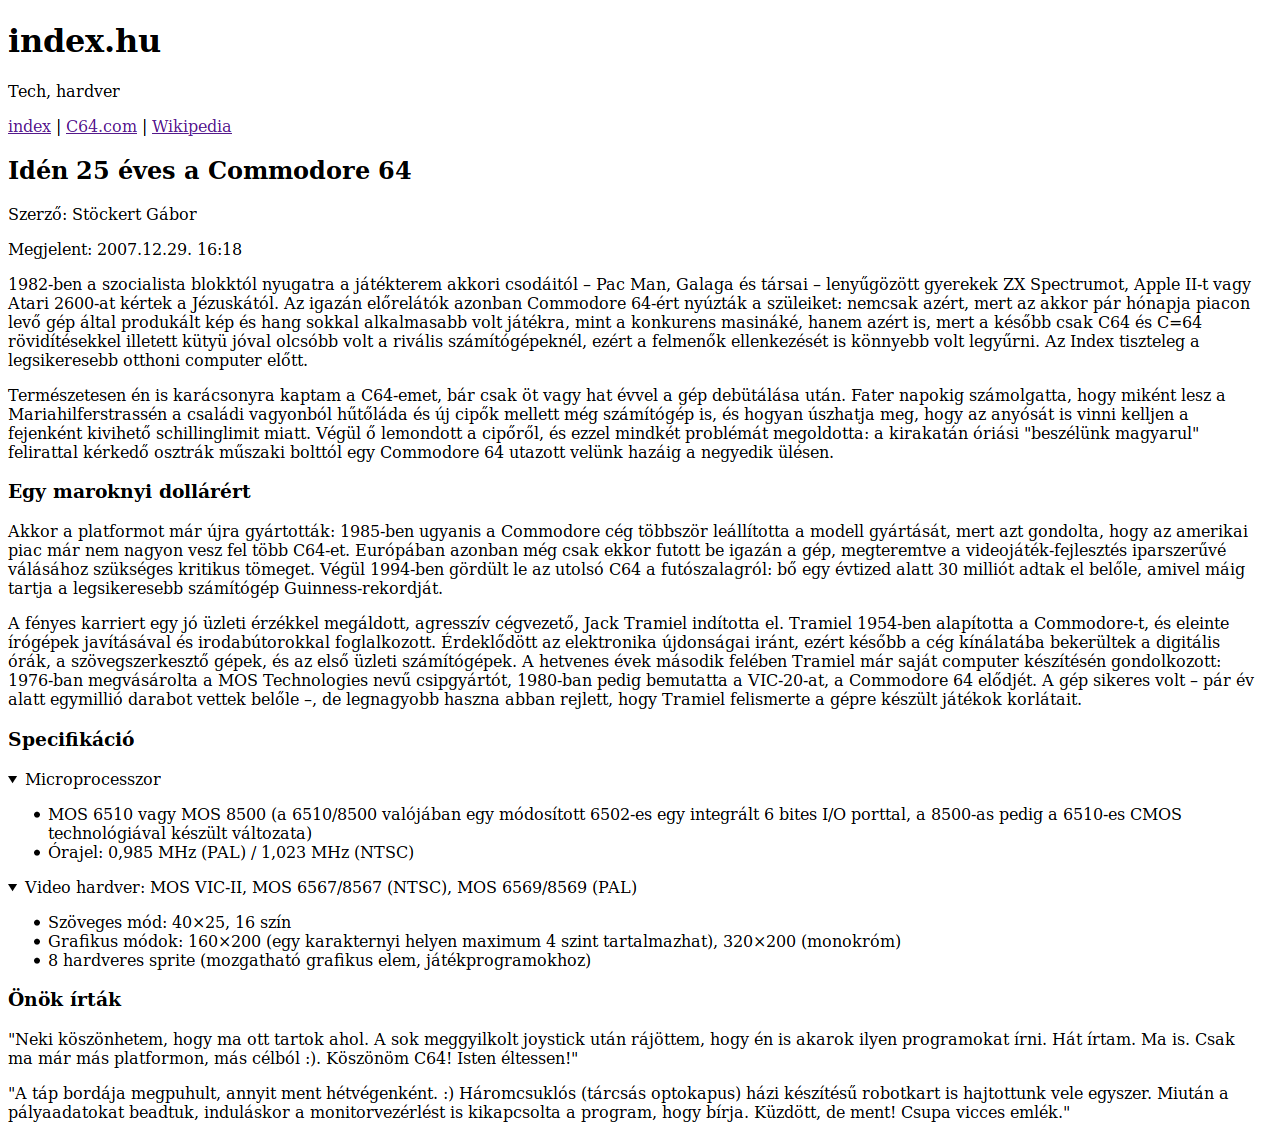
\includegraphics[scale=.14,]{c64.png}
  \end{exampleblock}
\end{frame}
